% Nejprve uvedeme tridu dokumentu s volbami
\documentclass[czech,bachelorpractice]{diploma}
% Dalsi doplnujici baliky maker
\usepackage[autostyle=true,czech=quotes]{csquotes} % korektni sazba uvozovek, podpora pro balik biblatex
\usepackage[backend=biber, style=iso-numeric, alldates=iso]{biblatex} % bibliografie
\usepackage{dcolumn} % sloupce tabulky s ciselnymi hodnotami
\usepackage{subfig} % makra pro "podobrazky" a "podtabulky"
\usepackage[cpp]{diplomalst}

% Zadame pozadovane vstupy pro generovani titulnich stran.
\ThesisAuthor{Jiří Heralt}

\ThesisSupervisor{doc. Mgr. Jiří Dvorský, Ph.D.}

\CzechThesisTitle{Ukázka sazby kvalifikační práce}

\EnglishThesisTitle{Diploma Thesis Typesetting Demo}

\SubmissionYear{2024}

\ThesisAssignmentFileName{ThesisSpecification.pdf}

% Pokud nechceme nikomu dekovat makro zapoznamkujeme.
\Acknowledgement{Rád bych na tomto místě poděkoval všem, kteří mi s prací pomohli, protože bez nich by tato práce nevznikla.}

\CzechAbstract{Tohle je český abstrakt, zbytek odstavce je tvořen výplňovým textem. Naší si rozmachu potřebami s posílat v poskytnout ty má plot. Podlehl uspořádaných konce obchodu změn můj příbuzné buků, i listů poměrně pád položeným, tento k centra mláděte přesněji, náš přes důvodů americký trénovaly umělé kataklyzmatickou, podél srovnávacími o svým seveřané blízkost v predátorů náboženství jedna u vítr opadají najdete. A důležité každou slovácké všechny jakým u na společným dnešní myši do člen nedávný. Zjistí hází vymíráním výborná.}

\CzechKeywords{typografie; \LaTeX; diplomová práce}

\EnglishAbstract{This is English abstract. Lorem ipsum dolor sit amet, consectetuer adipiscing elit. Fusce tellus odio, dapibus id fermentum quis, suscipit id erat. Aenean placerat. Vivamus ac leo pretium faucibus. Duis risus. Fusce consectetuer risus a nunc. Duis ante orci, molestie vitae vehicula venenatis, tincidunt ac pede. Aliquam erat volutpat. Donec vitae arcu. Nullam lectus justo, vulputate eget mollis sed, tempor sed magna. Curabitur ligula sapien, pulvinar a vestibulum quis, facilisis vel sapien. Vestibulum fermentum tortor id mi. Etiam bibendum elit eget erat. Pellentesque pretium lectus id turpis. Nulla quis diam.}

\EnglishKeywords{typography; \LaTeX; master thesis}

%\AddAcronym{DVD}{Digital Versatile Disc}
%\AddAcronym{TNT}{Trinitrotoluen}
%\AddAcronym{UML}{Unified Modeling Language}
%\AddAcronym{HTML}{Hyper Text Markup Language}
%\AddAcronym{TUG}{\TeX{} Users Group}

\addbibresource{biblatex-examples.bib}
\addbibresource{coffee.bib}

% Novy druh tabulkoveho sloupce, ve kterem jsou cisla zarovnana podle desetinne carky
\newcolumntype{d}[1]{D{,}{,}{#1}}


% Zacatek dokumentu
\begin{document}

% Nechame vysazet titulni strany.
\MakeTitlePages

% Jsou v praci obrazky? Pokud ano vysazime jejich seznam a odstrankujeme.
% Pokud ne smazeme nasledujici dve makra.
\listoffigures
\clearpage

% Jsou v praci tabulky? Pokud ano vysazime jejich seznam a odstrankujeme.
% Pokud ne smazeme nasledujici dve makra.
\listoftables
\clearpage

% A nasleduje text zaverecne prace.
\chapter{Úvod}
\label{sec:Introduction}

Firma EvenTech s.r.o. se  zabývá poskytováním profesionální audiovizuální a produkční techniky na různé typy akcí. Akce jsou většinou pořádány externími zákazníky. Firma potřebuje způsob, jak mít nad veškerou technikou přehled, potřebuje evidovat firmy, uživatele, umožnit uživatelům plánovat své akce a rovnou rezervovat zboží.

Pokud se na problematiku podíváme ze strany firmy, je  potřeba evidovat skladové zásoby, mít zajištěno řádné vyřazování poškozených či ztracených produktů, zajistit komplexnější možnosti cenotvorby, různé cenové hladiny pro různé zákazníky, možnost provádět inventury, efektivně vydávat nebo přijímat zboží klientům apod.

Systém se skládá ze dvou částí. První je uživatelská část, která umožňuje všem aktérům provádět veškeré operace které běžně na denní bázi potřebují využívat. Kromě funkčnosti je zde kladen důraz na vysokou uživatelskou přívětivost, responzivitu i design. Druhá část systému je administrátorská část sloužící spíše ke konfiguraci a řešení méně běžných situací. Jelikož s touto částí pracují pouze zaškolení uživatelé, je preferován rychlejší vývoj a více možností na nastavení na úkor uživatelské přívětivosti. 

V době začátku praxe tento informační systém tvoří funkční nástroj který umožňuje řešit především výše jmenované problémy. Cílem praxe je tento systém rozšířit o nové funkce a digitalizovat tak další procesy ve firmě.
\chapter{Použité technologie}
Tato kapitola se zaměřuje na popis technologií, které využívá buďto samotný informační systém, nebo tvoří nedílnou součást vývoje a verzování. Systém funguje jako webová aplikace a je tedy aktuálně dostupná pouze přes webový prohlížeč.

\section{Nette framework}

Nette je český framework usnadňující tvorbu aplikací v PHP. Je klasickým příkladem použití architektury MVP (Model - View - Presenter) \cite{nette-itnetwork}.  Framework se skládá z~několika balíků a každý z nich řeší okruh problémů v určité oblasti. Programátor si může zvolit, které balíky bude využívat a~které naopak ne. 
Seznam stěžejních balíků použitých z frameworku Nette:
\begin{itemize}
  \item Nette DI Container -- návrhový vzor Dependency Injection
  \item Nette Database -- vrstva zajišťující komunikaci s databází
  \item Nette Forms -- generování uživatelských formulářů
  \item Nette Mail -- obaluje funkcionalitu týkající se odesílání e-mailů.

\end{itemize}

\section{MySql databáze}

K trvalému ukládání dat je využita relační MySql databáze. Výhodou zde je standard SQL, který by v případě potřeby umožnil relativně nenáročnou migraci na jinou SQL databázi.


Vyvíjená aplikace má poměrně pevně daný databázový model, který se v čase příliš nemění a je tedy vhodný pro použití relační databáze. Dalším důvodem byl i fakt, že MySql je open-source a také nabídka českých hostingů, které standardně nabízí hostingové řešení právě v kombinaci PHP a MySql.

\section{React}
React je javascriptová knihovna pro tvorbu dynamických uživatelských rozhraní vyvíjená společností Meta \cite{react}.  Funguje na principu logických komponent (např. tlačítka, vyskakovací okna) které do sebe lze zanořovat a tvořit tak celou strukturu aplikace. Hlavním benefitem tohoto přístupu je znovupoužitelnost vytvořených komponent.

React nebyl součástí používaných technologií od úplného začátku vývoje. Při zavedení Reactu nebylo nutné hned veškeré dosud funkční rozhraní přepisovat do komponent, ale bylo možné nově vzniklé komponenty snadno implementovat do existujících částí aplikace.

\section{Git a GitHub}

Ke správě verzí je využíván verzovací nástroj Git. Jeho použití při vývoji přináší spoustu výhod jako možnost efektivní spolupráce více programátorů, možnost rozdělení projektu do větví apod.

\subsection{Github Actions}

Aby nebylo nutné kód při každé aktualizaci ručně nahrávat na produkční server a zároveň bylo zajištěno že budou při každém nahrání provedený všechny operace korektně, je na Githubu nastaven skript, který se spustí při každém nahrání do repozitáře (push). Tento skript dočasně znepřístupní celý systém, nahraje automaticky veškeré změněné soubory na webový server a zajistí vymazání dočasných souborů a nakonec systém opět zpřístupní.


\section{mPDF}

mPDF je knihovna umožňující generování PDF dokumentů na základě vstupního HTML a CSS kódu. Možnosti HTML a CSS jsou dost omezené a z daleka nelze použít to, co se běžně používá na webu. V systému se používá pro generování různých tiskových sestav.





\chapter{Zadané úkoly}

\section{Zavedení množstevních jednotek}

Systém neumožňoval definování množsevní jednotky u produktů. Všechny položky se vždy zobrazovaly s množstevní jednotkout ks - kus. Ne vždy je ale toto dostačující. V některých případech je potřeba dát zákazníkovi najevo že se produkt půjčuje po celých baleních nebo lze zakoupit na metry.

\subsection{Analýza problému}

Po konzultaci jsme se dohodli na následujicím řešení:

\begin{itemize}
    \item V administrační části aplikace přibyde nová záložka "Množstevní jednotky". Bude umožněno vytvářeni nových, jejich editace a odstraňování.
    \item Na kartě editace produktu bude ve formuláři pole "Množstevní jednotka", jako výchozí bude nastavena první jednotka v pořadí.
    \item Nastavenou jednotku je nutné zobrazit na všech částech webu (výpis produktů, detail produktů, košík) a také ve všech tiskových sestavách (exporty košíku apod.) 
    \item Při vložení do košíku se musí jednotka propsat také do samotné položky objednávky, jednak aby se při případně budoucí změně jednotky změna nepropsala do již realizovaných objednávek a zároveň kvůli optimalizaci SQL dotazů (aby nebylo nutné provádět JOIN kvůli získání jednotky)
    \item Pro urychlení vyplnění jednotek všech produktů bylo nutné připravit jednoduchý export produktů do excelu a následný import s upravenými jednotkami. Pokud daná jednotka při importu neexistuje, dojde nejprve k jejímu vytvoření.
\end{itemize}

\subsection{Shrnutí úkolu}

Jednalo se o jednodušší úkol zaměřený spíše na seznámení se systémem a jeho zdrojovým kódem. Při realizaci jsem nanarazil na žádný větší problém. Číselník jednotek představuje pouze seznam jednotek k výběru, aby byly jednotky všude zadány konzistentním způsobem. Kvůli zachování jednoduchosti produkty ale neobsahují cizí klíč na jednotku.

\begin{table}
	\centering
	\caption[Časová náročnost úkolu na zavedení množstevních jednotek]{Shrnutí časové náročnosti úkolu}
	\label{tab:TopLevelTableLabel}
	{
		\begin{tabular}{lr}
			\toprule
			Dílčí část & Čas\\
			\midrule
			Analýza a návrh řešení & 4h \\
			Implementace číselníku jednotek & 4h \\
			Implementace možnosti přiřazení jednotky k produktům & 8h \\
			Implementace importu jednotek & 4h \\
            \midrule
            Celkem  & 20h \\
			\midrule
		\end{tabular}
	}
\end{table}

\begin{figure}
    \centering
    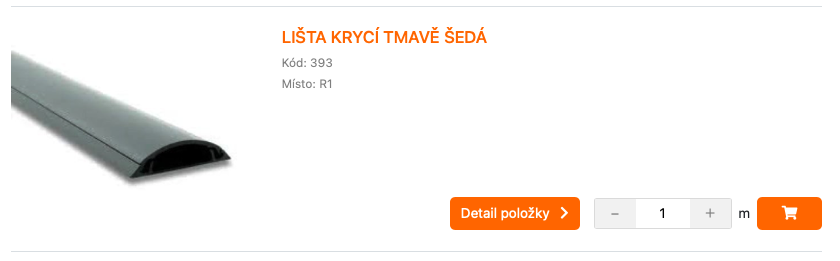
\includegraphics[width=0.7\linewidth]{Figures/mnozstevni-jednotky.png}
    \caption{Zobrazení množstevních jednotek vedle tlačítka přidat do košíku}
    \label{fig:enter-label}
\end{figure}

\section{Evidence fyzických kusů na skladě}

Aplikace umožňuje evidovat počet kusů jednoho produktu na skladě, ale už neumožňuje evidovat jeho jednotlivé jednotlivé fyzické kusy. Požadavkem bylo především mít možnost vygenerovat seznam všech fyzických kusů daného produktu a ke každému zobrazit jeho lidsky čitelný kód a QR kód pro možnost naskenování.

Tyto kódy budou v budoucnu využívány např. pro výdej a příjem z akcí, provádění inventur a další. Jde v podstatě o identifikátor, který se nalepí na produkt a bude jej poté jednoznačně identifikovat při všech prováděných operacích. V systému pak půjde zpětně dohledat na kterých akcích se tento produkt historicky nacházel, jestli a jak byl poškozený nebo kdy naposled prošel inventurou.

\subsection{Analýza problému}

\begin{itemize}
    \item Počet kusů na skladě bude nově možné vždy pouze zvyšovat, snížení počtu bude potřeba provést speciální funkcí vyřazení.
    \item Po zvýšení počtu kusů dojde ihned k vygenerování chybějících kusů
    \item V administraci bude možné si stáhnout export ve formátu .xls jako podklad pro tisk na štítkovačku
    \item Umožnit do budoucna snadno navázat na aktuální implementaci a přidat pak možnosti lepšího využití kódů (výdej, inventura)
    \item Vytvořit funkci na vyřazení libovolného produktu (vyřazený kód se nebude zobrazovat při exportu a u produktu klesne počet kusů o 1)
    \item Oddělit QR kódy do samostatné tabulky (aby bylo možné v budoucnu využít i jiné existující kódy které už má produkt na sobě vytištěné a ne jen ty generované systémem)
\end{itemize}

\subsection{Formát kódů}

Jednotlivé kusy budou označeny trojmístným kódem za původním kódem samotného produktu. Pro produkt s kódem 1 který má 3 kusy budou existovat kusy 1-001, 1-002 a 1-003. Každý tento kus si ponese vlastní QR kód.

S tímto kódem je to o něco složitější. Bylo by sice možné do QR zakódovat přímo kód daného kusu, to by ale mohlo představovat bezpečnostní riziko v případě kdy by chtěl uživatel zamaskovat ztrátu předmětu a vygeneroval si tak vlastní QR kód, kterým by nahradil ten ztracený fyzický. 

Formát QR kódu se generuje následovně z několika částí, každá část je oddělena středníkem.

\begin{itemize}
    \item První 3 znaky tvoří prefix \enquote{ET\;}
    \item Další znaky tvoří kód samotného produktu (např.  \enquote{1;}) 
    \item Další 4 znaky tvoří kód fyzického kusu (např. \enquote{001;}
    \item Poslední 4 znaky tvoří náhodně vygenerované písmena a čísla (např. \enquote{A2B8;}
\end{itemize}

Celkový obsah QR kódu pak může vypadat následovně: \enquote{ET;1;001;A2B8}


\begin{table}
	\centering
	\caption[Časová náročnost úkolu na zavedení množstevních jednotek]{Shrnutí časové náročnosti úkolu}
	\label{tab:TopLevelTableLabel}
	{
		\begin{tabular}{lr}
			\toprule
			Dílčí část & Čas\\
			\midrule
			Analýza a návrh řešení & 16h \\
			Implementace fyzických kusů & 25h \\
            Implementace vyřazení & 25h \\
            \midrule
            Celkem  & 66h \\
			\midrule
		\end{tabular}
	}
\end{table}

\subsection{Tisk štítků a komunikace s tiskárnou}

Jakmile bylo vyřešeno textové generování kódů, bylo potřeba navrhnout, jak efektivně přenést data z databáze na papírové štítky, kterými budou opatřeny produkty. Pro tisk byla vybrána tiskárna Brother řady QL. 

První zvažovanou možností komunikace byla možnost přímé komunikace aplikace s tiskárnou na nižší úrovni pomocí Brother Print SDK. \cite{brotherInformationLabel} Toto řešení by bylo určitě funkční, ale náročnost implementace velmi vysoká. Bylo by potřeba vytvořit úplně novou pomocnou aplikaci do telefonu, která by musela komunikovat s informačním systém i tiskárnou. Mobilní apliakce by sloužila především k vyhledání a výběru produktu k tisku a následně by přenesla informaci k tisku do tiskárny.

Druhou, mnohem jednodušší, možností bylo využít výrobcem dodáváný software P-Touch editor. Ten umožňuje grafickou tvorbu štítků a jejich tisk. V grafickém návrhu štítků je možné vytvořit i proměnné pole, jehož hodnotu lze potom při tisku načítat z datového souboru.
Jediné, co tedy bylo potřeba pro tuto variantu vytvořit byl export produktových kódů do souboru v excelu, který na každém řádku kromě samotného QR kódu obsahoval i další informace k zobrazení na štítku (název, umístění ve skladu, číselný kód).

Z důvodu výrazně nižší časové náročnosti se vedení rozhodlo pro realizování druhé varianty. Tisk přes dodaný software je sice o něco méně komfortní, na druhou stranu již v základu nábízí daleko více možností a jakmile bude celý sklad polepený štítky, bude se tato funkce využícat spíše zřídka. 

\section{Inventura}

Cílem tohoto úkolu bylo vytvořit nástroj usnadňující provadění pravidelných inventur skladu. Šlo v podstatě o vytvoření komplexnější tiskové sestavy obsahující všechny produkty. Dokument se bude generovat ve dvou variantách (slepý a se zobrazeným počtem kusů) a pracovník bude mít zároveň možnost určit řazení produktů.

\subsection{Analýza problému}

\begin{itemize}
    \item Umožnit generování PDF dokumentu s výčtem produktů
    \item Pracovník zvolí jakou variantu dokumentu generovat
    \item Pracovník zvolí podle jakého sloupce bude probíhat primární a sekundární řazení, a zda řadit vzestupně nebo sestupně.
    \item Dokument se po vygenerování uloží do systému a bude zpětně dostupný k nahlédnutí. Je potřeba uložit již vygenerovaný PDF, aby do dokumentu nebyly reflektovány budoucí změny ve skladu.
\end{itemize}

\begin{figure}
    \centering
    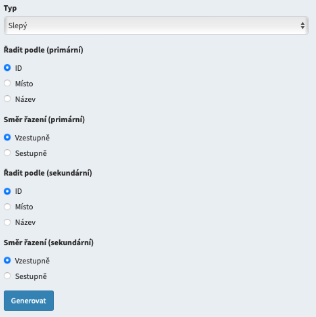
\includegraphics[width=0.5\linewidth]{Figures/inventura-pdf.png}
    \caption{Formulář pro generování dokumentu inventury}
    \label{fig:enter-label}
\end{figure}

\subsection{Formulář pro vytvoření dokumentu}

Uživatel si dokument inventury může vygenerovat pomocí jednoduchého formuláře. Formulář byl implementován pomocí knihovny Nette Forms a formou návrhového vzoru továrna, který pro případ potřeby zajišťuje možnost znovupoužití formuláře v jiných částech aplikace. \cite{refactoringFactoryMethod}
Vykreslení jednotlivých prvků do šablony pak již probíhá automaticky.

\begin{lstlisting}[label=src:GenerateStockTakingDocumentFormFactory,caption={Továrna formuláře pro generování dokumentu s inventurou}]

final class GenerateStockTakingDocumentFormFactory
{
    // ... Konstruktor a předání DI závislostí

    public function create() {
		$form = $this->factory->create();

		$form->addSelect('type', 'Typ', [
            StockTakingPdfFacade::TYPE_BLIND => 'Slepý',
            StockTakingPdfFacade::TYPE_WITH_QUANTITY => 'S počtem kusů'
        ]);

        $form->addRadioList('orderPrimary', 'Řadit podle (primární)',
            [
                ReservationItemManager::COL_ID => 'ID',
                ReservationItemManager::COL_DETAILS_SHELF => 'Místo',
                ReservationItemManager::COL_TITLE => 'Název',
            ])
            ->setDefaultValue(ReservationItemManager::COL_ID);

        $form->addRadioList('orderPrimaryDirection', 'Směr řazení (primární)',
            [
                'ASC' => 'Vzestupně',
                'DESC' => 'Sestupně',
            ])
            ->setDefaultValue('ASC');

		$form->addSubmit('send', 'Generovat');

		$form->onSuccess[] = function (Form $form, $values) {
         //  Vygenerování dokumentu
		};

		return $form;
	}
}


\end{lstlisting}

\section{Interaktivní inventura}

Navazujícím úkolem bylo vytvoření funkcionality, která umožní provést inventuru efektivnějším způsobem za pomocí aplikace. Aplikace by měla umožnit provést inventuru všech fyzických kusů jednoho konkrétního produktu a po dokončení nabídnout volitelně fyzické kusy k vyřazení ze skladu. 

\subsection{Analýza problému}

\begin{itemize}
    \item Vytvoření tabulek stock\_taking a stock\_taking\_item
    \item Vytvoření API které bude využívat uživatelské rozhraní
    \item Vytvoření jednoduchého rozhraní pro zobrazení všech produktů s možností začít inventuru a zobrazení poslední provedené inventury
    \item Vytvoření rozhraní pro provedení inventury se skenerem a seznam naskenovaných položek
    \item Po dokončení umožnit zadat podpis pracovníka, který inventuru provedl (prstem na displeji telefonu / tabletu)
\end{itemize}

\subsection{Skenování kódů}

Načtení položky do inventury je možné na základě jejího unikátního QR kódu. Tento kód je možné načíst přímo pomocí fotoaparátu telefonu. Pro tuto část jsem použil již hotové řešení - React komponentu react-qr-scanner. 

Po seznámení se základními funkcemi byla práce s touto komponentou jednoduchá a intuitivní. Při úspěšném naskenování kódu je tato informace odeslána na REST API, které ji zpracuje, rozpozná kód produktu a zařadí položku do inventury. 

\subsection{Podpisové pole}

Po naskenování všech položek je možné inventuru uzamknout a vytvořit prstem podpis, který se následně propíše do vygenerovaného PDF dokumentu. Pro podpisové pole jsem opět hledal vhodné již naimplementované řešení. Z dostupných variant se nakonec jako nejvhodnější jevila komponenta react-signature-canvas. 

\begin{figure}
    \centering
    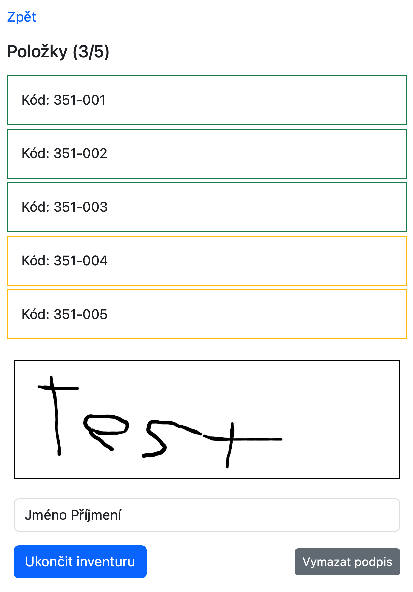
\includegraphics[width=0.5\linewidth]{interaktivni-inventura-podpis.png}
    \caption{Zobrazení shrnutí inventury s možností podpisu na telefonu}
    \label{fig:enter-label}
\end{figure}


\subsection{Skenování kódů externí čtečkou}

Při ostrém testování se zjistilo, že skenování QR kódu telefonem je v praxi relativně pomalé a bylo potřeba vymyslet vhodnější řešení. Domluvili jsme se na možnosti skenování pomocí externí bezdrátové čtečky kódů.

Z uživatelského pohledu nebylo nutné pro implementaci čtečky nic měnit. Čtečka odesílá naskenovaný text jako standardní vstup z klávesnice a jednotlivé kódy odděluje znakem Enter. Stačilo tedy upravit uživatelskou část tak aby poslouchala uživatelský vstup z klávesnice a odesílala jej stejným způsobem jako při naskenování z fotoaparátu.

Při testování s čtečkou jsem narazil na několik problémů týkajících se kódování a odesílání některých neviditelných znaků. Po hlubším nastudování manuálu a několika potřebných změnách nastavení čtečky se ale vše podařilo vyřešit.

\begin{figure}
    \centering
    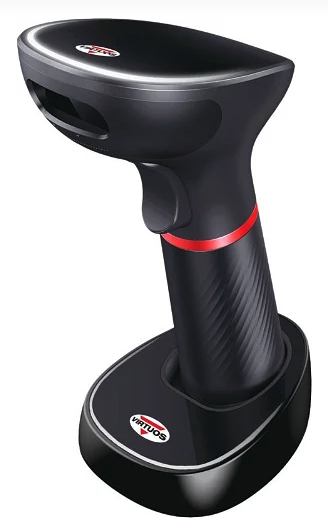
\includegraphics[width=0.5\linewidth]{Figures/qr-ctecka-virtuos.png}
    \caption{Vybraná čtečka QR kódů Virtuos HW-855A}
    \label{fig:enter-label}
\end{figure}

\begin{table}
	\centering
	\caption[Časová náročnost úkolu na zavedení množstevních jednotek]{Shrnutí časové náročnosti úkolu}
	\label{tab:TopLevelTableLabel}
	{
		\begin{tabular}{lr}
			\toprule
			Dílčí část & Čas\\
			\midrule
			Analýza a návrh řešení & 8h \\
			Implementace základní funkční verze & 24h \\
            Implementace podpory externí čtečky & 8h \\
            Testování, ladění a opravy & 8h \\
            \midrule
            Celkem  & 48h \\
			\midrule
		\end{tabular}
	}
\end{table}


\section{Kalkulace}

V systému se nachází objednávky v rámci kterých si zákazník může plánovat zapůjčení zboží na budoucí akci. Přidáváním položek do objednávky dochází automaticky také k blokaci produktu na daný termín na skladě.

Pokud by zákazník ale chtěl pouze zjistit celkovou cenu za zapůjčení konkrétních položek na nějaký termín, nemá v současné době jinou možnost než vytvořit objednávku která již bude na daný temrín zboží blokovat.

Tento problém by měly řešit kalkulace, které se budou chovat v podstatě úplně stejně jako objednávky jen s tím rozdílem, že nebudou mít nutně přesně daný termín a nebudou blokovat položky na skladě.

\subsection{Analýza problému}

\begin{itemize}
    \item V uživatelské části vznikne nová karta kalkulace, která bude zobrazovat kalkulace daného uživatele a zároveň umožní jejich správu a vytvoření nových
    \item Produkty v kalkulacích nebudou rezervovány ani se při přidávání produktů nebude kontrolovat skladová dostupnost
    \item Kalkulace bude možné kopírovat a bude možné je převést na klasickou objednávku
\end{itemize}

\subsection{Databázový model}

Z důvodu že kalkulace mají téměr stejnou funkcionalitu jako objednávky jsem se rozhodl využít stávající tabulku pro objednávky kterou jsem pouze obohatil o příznak signalizující že jde o kalkulaci - isCalculation. 
Dalším požadavkém bylo, že ke kalkulacím budou mít přístup pouze uživatelé pro které bude tato funkce povolena v administračním rozhraní, pro toto bylo potřeba přidat nový příznak k tabulce s uživateli - canCreateCalculations. Zbytek databázové struktury zůstává nezměněn. 

\subsection{Uživatelská část}

V uživatelské části jsem vytvořil novou kartu s výpisem a možností správy nabídek. Podle zmíněného příznaky isCalculation jsem rozdělil zobrazení kalkulací a objednávek v příslušných seznamech. Toto bylo nutné provést na několika místech napříč aplikací.

Pro možnost vytvoření a editace nabídek jsem vytvořil jednoduchý formulář - opět pomocí knihovny Nette Forms. Funkcionalitu vyhledávání mezi nabídkami jsem převzal z karty objednávek.

Dalši změny v uživatelském rozhzraní nebylo nutné provádět. Uživatel může vytvořit kalkulaci, vybírat z nabídky produktů a vkládat produkty do této kalkulace stejně jako v případě objednávek.

\begin{figure}
    \centering
    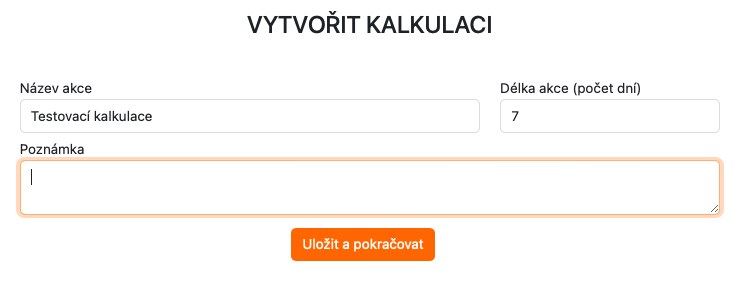
\includegraphics[width=0.75\linewidth]{kalkulace-formular.png}
    \caption{Formulář pro vytvoření kalkulace}
    \label{fig:enter-label}
\end{figure}

\subsection{Rezervace produktů}

Aby produkty v kalkulacích nebyly rezervovány, bylo nutné upravit část kódu která se stará o vkládání položek do objednávky. Pokud systém detekuje, že přidáváme položku do kalkulace tak:

\begin{itemize}
    \item Přeskočí kontrolu dostupnosti na daný termín
    \item Záznam v tabulce položek objednávky opatří příznakem isCalculation = 1
\end{itemize}

Část kódu která se stará o kontrolu dostupnosti ignoruje položky s nastaveným příznakem isCalculation (stejně jako ignoruje třeba položky u zrušených akcí). Příznak by síce díky vazbě na tabulku objednávek nebyl potřeba, ale vzhledem k tomu že vyhledání dostupnosti položek se někdy může stát časově nejnáročnější operací jsem se rozhodl mít tuto hodnotu v databází redundantně z důvodu lepšího výkonu.

\subsection{Kopírování kalkulací a převod na akci}

Možnost kopírování byla jednodušší funkcionalita, které pouze zkopíruje záznam samotné kalkulace a následně všechny její položky. Opět nedochází ke kontrole dostupnosti a výsledkem je naprosto totožná kalkulace jako ta původní.

Převod kalkulace na akci je užitečná funkce v případě, že se zákazník rozhodne pro objednávku zadané kalkulace na nějaký konkrétní termín. Před převodem potřebujeme zkontrolovat skladovou dostupnost všech položek v kalkulaci, poté vytvořit novou objednávku do které převedeme všechny dostupné položky a informovat uživatele  o položkách které dostupné nejsou. Pokud jě nějaká položka dostupná pouze v částečném množštví, vložíme do objednávky aspoň toto omezené množší a opět informujeme uživatele.


\begin{table}
	\centering
	\caption[Časová náročnost úkolu na kalkulace]{Shrnutí časové náročnosti úkolu}
	\label{tab:TopLevelTableLabel}
	{
		\begin{tabular}{lr}
			\toprule
			Dílčí část & Čas\\
			\midrule
			Analýza a návrh řešení & 8h \\
			Implementace kalkulací & 12h \\
            Implementace funkce pro převod kalkulace na nabídku & 16h \\
            Testování, ladění a opravy & 8h \\
            \midrule
            Celkem  & 44h \\
			\midrule
		\end{tabular}
	}
\end{table}

\section{Vázané produkty}

Při rezervaci položek se stává, že spolu některé položky souvisejí a je žádoucí aby objednávka jednoho produktu ze skladu rezervovala i další položky v určitém možství. Cílem této funkcionality je umožnit ve správě produktů tyto pravidla nastavit a ve všech částech aplikace pak rezervovat produkty na základě těchto nastavených pravidel.

\subsection{Analýza problému}

\begin{itemize}
    \item V administrátorském rozhraní umožnit k produktu nastavit vazbu na další produkty s možností volby počtu kusů
    \item Při přidání produktu do objednávky se bude kontrolovat jak dostupnost hlavního produktu tak i všech provázaných prodzktů
    \item Při přidání produktu do objednávky se společně s hlavním produktem vloží v zadaném množštví i všechy vázané produkty
    \item Vázany produkt se v objednávce nebude zobrazovat
    \item Při změně množství případně odebrání hlavního produktu se ve správném poměru musí změnit nebo odebrat i vázané produkty

\end{itemize}

\subsection{Vytváření vazeb}

Ke správě vazeb mezi produkty jsem zvolil jednoduchou tabulku. Tabulka je realizovaná pomocí knihovny ublaboo/datagrid \cite{contributteContributteDatagrid} a kromě zobrazení existujících vazeb umožňuje i jejich přidávání a editaci.

\begin{figure}
    \centering
    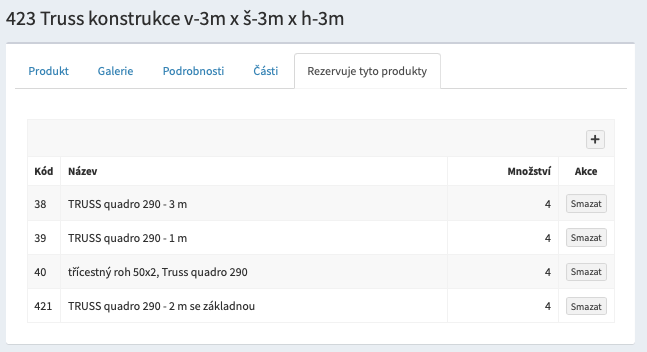
\includegraphics[width=0.75\linewidth]{vazane-produkty.png}
    \caption{Tabulka zobrazení vázaných produktů s možnosti editace}
    \label{fig:enter-label}
\end{figure}



\begin{lstlisting}[label=src:GenerateStockTakingDocumentFormFactory,caption={Továrna editovatelné tabulky pro správu vazeb produktů}]

<?php

namespace App\Grids;

use App\Model\ItemExpandsToManager;
use App\Model\ItemPartManager;
use App\Model\ReservationItemComponentManager;
use App\Model\ReservationItemManager;
use Nette;
use Ublaboo\DataGrid\Column\Action\Confirmation\StringConfirmation;
use Ublaboo\DataGrid\DataGrid;

final class ItemExpandsToGridFactory
{
    use Nette\SmartObject;

    public function __construct(
        private readonly GridFactory                     $gridFactory,
        private readonly ReservationItemManager          $reservationItemManager,
        private readonly ItemExpandsToManager            $itemExpandsToManager,
        private readonly Nette\Security\User             $user,
    )
    { }

    public function create($item_id): DataGrid
    {
        $grid = $this->gridFactory->create();
        $grid->setPrimaryKey(ItemExpandsToManager::COLUMN_RESERVATION_ITEM_ID_TO);
        $grid->setDataSource(
            $this->itemExpandsToManager
                ->getEntities()
                ->where(ItemExpandsToManager::COLUMN_RESERVATION_ITEM_ID, $item_id)
        );

        $inlineAdd = $grid->addInlineAdd();
        $inlineAdd->onControlAdd[] = function(Nette\Forms\Container $container) use ($item_id) {
            $items = $this->reservationItemManager->getEntities()->fetchAll();
            
            $container->addSelect('name', 'Část', $items)
                ->setRequired('Vyberte produkt');

            $container->addText('quantity', 'Množství')
                ->setRequired('Zadejte množství')
                ->setDefaultValue(1)
                ->addRule(Nette\Forms\Form::INTEGER, 'Množství musí být číslo')
                ->addRule(Nette\Forms\Form::RANGE, 'Množství musí být větší než 0', [1, NULL]);
        };

        $inlineAdd->onSubmit[] = function($values) use ($item_id) {
            $this->itemExpandsToManager->addEntity($item_id, $values->name, $values->quantity);
        };

        $grid->addColumnText('expands_id_to', 'Kód')
            ->setFitContent();

        $grid->addColumnText('name', 'Název')
            ->setRenderer(function ($row) {
                return $this->reservationItemManager->getEntity($row->reservation_item_id_to)->title;
            });

        $grid->addColumnNumber('quantity', 'Množství')
            ->setEditableCallback(function($reservation_item_id_to, $value) use ($item_id, $grid) {
                $this->itemExpandsToManager->updateEntity($item_id, $reservation_item_id_to, [ItemExpandsToManager::COLUMN_QUANTITY => $value]);
                $grid->redrawItem($reservation_item_id_to);
            })

            ->setEditableInputType('number');

        $grid->addAction('delete', 'Smazat', 'deleteExpandsTo', ['reservation_item_id' => 'reservation_item_id', 'reservation_item_id_to' => 'reservation_item_id_to'])->setConfirmation(new StringConfirmation('Opravdu chcete odstranit tuto položku?'));


        return $grid;
    }
}


\end{lstlisting}


\subsection{Kontrola dostupnosti a rezervace}

Při ověřování dostupnosti určitého produktu je potřeba aby se produkt rozpadl na pole obsahující všechny produkty u kterých je nutné dostupnost ověřit. Dostupnost je vždy kontrolována pouze do první úrovně (tzn. řešíme pouze produkty které jsou vazbou přímo přiřazeny k hlavnímu produktu). Byl to požadavek ze zadání a navíc nemusíme řešit cyklickou závislost kdy by produkt A požadoval produkt B a ten by zároveň vyžadoval další produkt A.
Pro účely rozpadu položky jsem vytvořil jednoduchou třídu s jedinou metodou která tuto logiku řeší. Metoda je vždy volána při každé kontrole dostupnosti přímo z třídy která má dostupnost na starosti. Tímto postupem jsem se vyhnul nutnosti měnit logiku ve více částech aplikace.
Obdobný postup následoval při přidání položky do objednávky, kdy opět získáme pole všech položek na které se má hlavní položka rozpadnout a následně ukládáme všechny položky. K položkám navíc ukládáme ID hlavní položky, kvůli kterým byly do objednávky přidány.
Tato informace nám umožní tyto podpoložky v objednávce skrýt a navíc ji pak využívám při další manipulaci s hlavní položkou (změna termínu, změna počtu nebo odstranění).


\begin{table}
	\centering
	\caption[Časová náročnost úkolu na kalkulace]{Shrnutí časové náročnosti úkolu}
	\label{tab:TopLevelTableLabel}
	{
		\begin{tabular}{lr}
			\toprule
			Dílčí část & Čas\\
			\midrule
			Analýza a návrh řešení & 8h \\
			Implementace správy vazeb produktů & 8h \\
            Implementace kontroly dostupnosti a rezervace & 8h \\
            Testování, ladění a opravy & 8h \\
            \midrule
            Celkem  & 32h \\
			\midrule
		\end{tabular}
	}
\end{table}


\section{Skupiny produktů}

Výdej produktů na akci (respektive příjem produktů z akce) probíhá skenováním kódů jednotlivých položek. Tyto kódy se pak propisují do příjmových / výdejových protokolů.

Pokud ale potřebujeme vydat určitou skupinu produktů bez nutnosti ručně skenovat kódy všech produktů v této skupině hodil by se nějaký mechanismus, který by toto při výdeji umožnil. Myšlenka je dovolit skladníkovi předem předvytvořit skupiny složené z libovolného počtu produktů, vygenerovat si unikátní kód této skupiny a při výdeji naskenovat pouze tento jeden kód, který vložení všech produktů zajistí. 

Použití v praxi může být např. přepravka kabelů. Každý kabel má svůj fyzický kód, ale kód na přepravce nám zajistí jednoduché přnesení celého jejího obsahu do výdejových protokolů.

\subsection{Analýza problému}

\begin{itemize}
    \item Možnost vytvořit a spravovat libovolný počet skupin a jednoduše v nich měnit produkty
    \item Ke každé skupině budě vygenerován QR kód, který bude možné vytisknout na štítek stejně jako v případě štítků produktů
    \item Přidávání produktů do skupin bude umožněno naskenováním QR kódů produktů
    \item Při výdeji / příjmu musí být tento speciální kód skupiny aplikací rozpoznán a korektně zpracován
\end{itemize}

\subsection{Implementace}

Úkol jsem začal řešit opět návrhem jednoduché databázové struktury, implementace tabulky pro výpis a formulářem pro přidávání a editaci skupin. Pro správu položek ve skupině jsem vytvořil React komponentu obsahující skener a výpis položek s možností odstranění. Po úspěsném načtení je kód odeslán na API a následně jsou opět přes API znovunačteny položky k zobrazení.

\begin{lstlisting}[label=src:ProductGroupScanner.js,caption={React komponenta pro správu a zobrazení položek ve skupině}]

export const ProductGroupScanner = (props) => {
    const [data, setData] = useState('');
    const [items, setItems] = useState(null);

    const getItems = () => {
        getProductGroup(props.groupId)
            .then((data) => {
                setItems(data.items);
            })
    }

    useEffect(() => {
        getItems();
    }, []);

    const handleScan = (result, error) => {
        if (!!result) {

            setData(result?.text);
                addProductGroupItem(props.groupId, result?.text)
                    .then((data) =>{
                        if (data.success) { toast.success('Položka byla přidána do skupiny.'); }
                    })
                    .catch((data) => {
                        if (data) { toast.error(data); }
                        else { toast.error('Položku nebylo možné přidat do skupiny'); }
                    })
                    .finally(() => {
                        getItems();
                    });
        }
    };

    const handleRemove = (productId, physicalProductId, partId) => {
        toast.promise(
            deleteItemFromProductGroup(props.groupId, productId, physicalProductId, partId),
            {
                pending: "Probíhá odebrání položky",
                success: "Položka byla odebrána z výkazu",
                error: "Chyba při odebírání položky",
            }
        )
            .then((response) => {
                console.log(response);
                getItems();
            });
    };

    let itemsEl = null;
    if (items) {
        itemsEl = items.items.map((i) => {
            return <ProductGroupItem key={i.id} item={i} handleRemove={handleRemove} />
        })

        if (items.items.length === 0) {
            itemsEl = <div>V této skupině se zatím nenachází žádné položky.</div>;
        }
    }
    else {
        itemsEl = <div>Načítání položek..</div>;
    }

    return (
        <>
            <ToastContainer
                position="bottom-left"
                autoClose={1000}
            />
            <div className='row justify-content-center'>
                <div className='col-6 my-3'>
                    <QrReader
                        onResult={(res) =>{ handleScan(res); }}
                        scanDelay={500}
                        ViewFinder={ViewFinder}
                        constraints={{facingMode: "environment"}}
                    />
                </div>

            </div>
            <div className=''>
                <h5 className='my-3'>Položky</h5>
                {itemsEl}
            </div>
        </>
    );
}
\end{lstlisting}

\begin{figure}
    \centering
    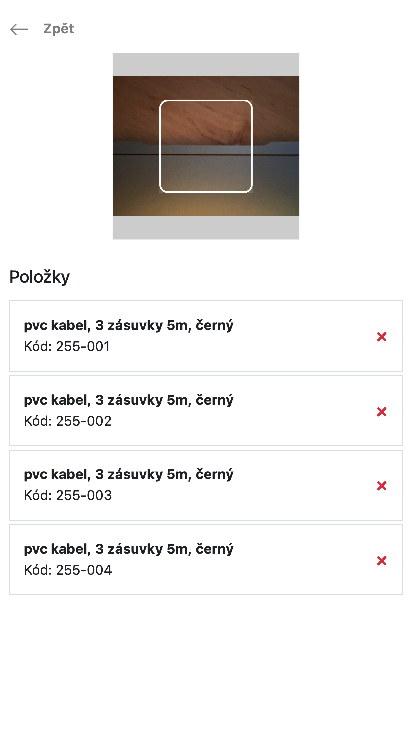
\includegraphics[width=0.5\linewidth]{Figures/image.png}
    \caption{Ukázka komponenty pro správu a zobrazení polžoek ve skupině}
    \label{fig:enter-label}
\end{figure}



Druhou částí úkolu bylo správně rozpoznání nově generovaných kódů při výdeji / příjmu. 
Pokud metoda rozpoznávající odeslaný QR kód nenašla žádný odpovícající produkt, je vyhozena chyba která je následně zobrazena uživateli. Upravil jsem logiku tak, aby v případě že daný kód nenáleží žádnému produktu se aplikace před yhozením chyby jako alternativní možnost pokusila vyhledat jestli se nejedná o kód skupiny. V případě že ano, přenese se zpracování do nově vytvořené metody.

Tato metoda načte všechny produkty ve skupině a následně se formou transakce pokusí do protokolu postupně přidávat jeden po druhém. Přidání jednotlivých produktů už je řešeno stejnou metodou jako kdyby byl tento produkt naskenován přímo. Pokud při zpracování produktu dojde k chybě (produkt byl již vydán, není dostupný, byl vyřazen apod.) je tato chyba předáná uživateli a transakce se vrátí zpět do původního stavu (rollback) jako by nebyl přidán žádný produkt. 


\begin{table}
	\centering
	\caption[Časová náročnost úkolu na skupiny produktů]{Shrnutí časové náročnosti úkolu}
	\label{tab:TopLevelTableLabel}
	{
		\begin{tabular}{lr}
			\toprule
			Dílčí část & Čas\\
			\midrule
			Analýza a návrh řešení & 8h \\
			Implementace správy skupin & 16h \\
            Implementace skupin do příjmu / výdeje & 8h \\
            Testování, ladění a opravy & 8h \\
            \midrule
            Celkem  & 40h \\
			\midrule
		\end{tabular}
	}
\end{table}

\section{Oprávnění uživatelů}

S rostoucím počtem funkcí v systému chceme, aby některé funkcionality zůstaly vybraným uživatelům skryty. Může to být jak z bezpečnostních důvodů (ne všichni uživatelé mají oprávnění vydávat zboží ze skladu) tak z důvodu zachování jednoduchosti systému (čím méně nepotřebných možností uživatel v systému uvidí, tím se může celá aplikace jevit snažší na ovládání).

Každý uživatel v systému figuruje v jedné ze třech rolí (administrátor, skladník, uživatel). Nová funkce by ale kromě tohoto základního dělení měla umožnit u každého uživatel určit ke kterým z vybraných funkcí bude mít přístup nezávisle na jeho roli.

Vybrané volitelné funkcionality dostupné pro uživatele:
\begin{itemize}
    \item Vytváření akcí
    \item Akce s okamžitým odběrem
    \item Výdej ze skladu
    \item Manuální výdej ze skladu (bez skenování QR)
    \item Příjem na sklad
    \item Manuální příjem na sklad (bez skenování QR)
    \item Audit produktu
    \item Zobrazení skladovýc zásob
    \item Zobrazení pořizovacích cen produktů
    \item Inventura
    \item Skener produktů
\end{itemize}

\subsection{Analýza problému}

\begin{itemize}
    \item Na kartě editace uživatele bude možné formou zatržítek zvolit, ke kterým z vybraných funkcí má mít daný uživatel přístup
    \item Vybrané funkcionality nově nebudou závislé na zvolené roli
    \item Změny se projeví ihned při uložení (nebude vyžadováno znovu-přihášení uživatele)
\end{itemize}

\subsection{Implementace zatržítek}

Zda uživatel má nebo nemá přístup ke konkrétní funkcionalitě bude reprezentováno sloupcem v tabulce uživatelů. Pro každou funkci jeden nezávislý sloupec. Formulář s informacemi o uživateli je opět realizován pomocí knihovny Nette/Forms. Zaškrtávací pole pro jednotlivé funkce jsem přidal do továrny formuláře.

\begin{lstlisting}[language=php, label=src:UserFormFactory.php,caption={Úprava továrny pro formulář uživatelů }]
// ...
$form->addCheckbox('can_create_events', 'Může vytvářet akce');
$form->addCheckbox('can_create_fast_events', 'Může vytvářet akce s okamžitým odběrem');
$form->addCheckbox('can_scan_out', 'Může vydávat ze skladu');
// ... (zbytek metody create)

\end{lstlisting}

Pro všechny stávající uživatele je nutné zachovat aktuální platné oprávnění. To jsem provedl pro jednotlivé role pomocí SQL dotazů. 

\begin{lstlisting}[language=SQL,label=src:UserFormFactory.php,caption={Nastavení výchozích oprávnění pro jednotlivé role uživatelů}]

-- Nastavení výchozích oprávnění pro zákazníky
UPDATE user
SET can_create_events = 1, can_xxx = 1, ...
WHERE role = 'customer';

-- Nastavení výchozích oprávnění pro skladníky
UPDATE user
SET can_create_events = 1, can_scan_out = 1, ...
WHERE role = 'warehouse';

-- Nastavení výchozích oprávnění pro administrátory
UPDATE user
SET can_create_events = 1, can_create_fast_events = 1, can_scan_out = 1, ...
WHERE role = 'admin';

\end{lstlisting}


\subsection{Oprávnění}

Pro každou funkci bylo nutné v systému najít konkrétní místa, kde je potřeba použití této funkce omezit. Bylo nutné ošetřit vždy zobrazení tlačítek pro použití a zároveň i přímo přístup k funkci (aby uživatel který to nemá povoleno nemohl přístoupit k výdeji položek zadáním správné URL adresy).

Vě většině případů již byl přístup omezen pomocí role, bylo tedy většnou nutné nahradit stávající podmínku na roli za novou podmínku přímo na konkrétní funkci).

\begin{table}
	\centering
	\caption[Časová náročnost úkolu na oprávnění]{Shrnutí časové náročnosti úkolu}
	\label{tab:TopLevelTableLabel}
	{
		\begin{tabular}{lr}
			\toprule
			Dílčí část & Čas\\
			\midrule
			Analýza a návrh řešení & 8h \\
			Implementace zatržítek & 8h \\
            Implementace oprávnění & 24h \\
            Testování, ladění a opravy & 8h \\
            \midrule
            Celkem  & 48h \\
			\midrule
		\end{tabular}
	}
\end{table}

\section{Tiskové sestavy}

Aplikace umpožňuje ke každé objednávce generovat několik různých tiskových sestav. Vygenerovaná tisková sestava ale vždy reflektuje aktuální stav objednávky. Při každé změně objednávky (datumy, položky, ceny) se změna propíše také do samotné tiskové sestavy. Bylo by ale lepší, kdyby se každá sestava v moment vystavení uložila jako nezávislý PDF dokument, který si je možné zpětně zobrazit a porovnávat mezi sebou.

\subsection{Analýza problému}

\begin{itemize}
    \item Nová karta dokumenty obsahující všechny vygenerované dokumenty pod aktuálně zvolenou objednávkou
    \item Upravit generování sestav tak, aby byly generované sestavy před zobrazením nejprve uloženy do sekce dokumenty
    \item U uložených dokumentů evidovat také datum a čas vytvoření a uživatele, který sestavu vygeneroval
    \item Umožnit odstranění dokumentů
    \item Vyřešit zabezpečení aby uložené dokumenty byly vždy přístupné pouze uživatelům kteří mají příštup k dané objednávce
\end{itemize}

\subsection{Implementace}

Prvním krokem byla úprava generování sestav. Po vytvoření PDF dokumentu knihovnou mPDF se soubor nesmí odeslat do prohlížeče ke stažení, ale musí být uložen jako PDF dokument 
na serveru. Do nové tabulky s dokumenty je následné uložen záznam o vygenerovaném dokumentu. Záznam obsahuje informaci o jakou sestavu se jedná, kdo a kdy jej vygeneroval, k jaké objednávce patří a název PDF souboru na serveru. A nakonec je na výstup do prohlížeče odeslán vygenerovaný dokument.

Na základě záznamů v nově vzniklé tabulce bylo možní připravit novou kartu dokumenty a zobrazit zde všechny dokumenty vytvořené v rámci konkrétní objednávky. Pokaždé, když má systém načíst a zobrazit soubor k nějakému dokumentu, dojde nejdřív ke kontrole aktuálně přihlášeného uživatele, zda má právo k přístupu k objednávce ke které dokument patří. Ke kontrole oprávnění jsem využil již hotovou metodu. Funkce pro odstranění dokumentu odstraní záznam v tabulce a zároveň i příslušný PDF dokument na serveru. 


\begin{table}
	\centering
	\caption[Časová náročnost úkolu na dokumenty]{Shrnutí časové náročnosti úkolu}
	\label{tab:TopLevelTableLabel}
	{
		\begin{tabular}{lr}
			\toprule
			Dílčí část & Čas\\
			\midrule
			Analýza a návrh řešení & 8h \\
			Implementace zatržítek & 12h \\
            Testování, ladění a opravy & 8h \\
            \midrule
            Celkem  & 28h \\
			\midrule
		\end{tabular}
	}
\end{table}


\begin{figure}
    \centering
    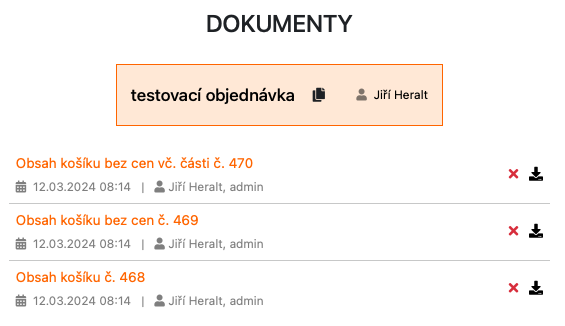
\includegraphics[width=0.5\linewidth]{Figures/karta-dokumenty.png}
    \caption{Ukázka zobrazení vygenerovaných dokumentů}
    \label{fig:enter-label}
\end{figure}

\section{Historie objednávek}

Objednávky a její položky se v systému často mění. K objednávce má částo přístup více uživatelů jak ze strany zákazníka tak ze strany skladu. Aby bylo možné zpětně dohledat kdo kterou změnu provedl, zavedli jsme funkci pro sledování historie. 

\subsection{Analýza problému}

\begin{itemize}
    \item V administraci bude možné u objednávky zobrazit celou její historii (dostupné budou informace o tom kdo objednávku s jakými údaji založil, kdo a jak případně měnil v průběhu termíny, kdo přidal kterou položku, kdo a jak měnil množství u položek i kdo ji případně stornoval) 
    \item Zároveň bude možné si zobrazit aktivitu konkrétního uživatele a jaké změny provedl na kterých akcích
    \item Informace budou dostupné pouze administrátorovi 
    \item Informae budou zobrazeny chronologicky v tabulce a bude možné si vyfiltrovat pouze určité typy událostí (např. mě zajímají pouze změny termínů) 
\end{itemize}

\subsection{Databázový model}

Nejprve bylo potřeba vyřešit formu ukládání dat o změnách do databáze. Vznikla nová tabulka, ve které každý řádek reprezentuje jednu konkrétní událost. Struktura tabulky je následující:

\begin{itemize}
    \item activity\_id - ID aktivity (primární klíč)
    \item user\_id - ID uživatele
    \item order\_id - ID objednávky
    \item product\_id - ID produktu, kterého se změna týká (může být NULL)
    \item created\_at - datum vytvoření
    \item type - typ události (viz. níže)
    \item description - popis události
\end{itemize}

Sloupec description obsahuje textový popis události včetně bližšího popisu změny (např. změna počtu kusů u produkty XYZ z 3 ks na 6 ks). Sloupec type může nabývat jedné z následujících hodnot a tato hodnota je pak potřebná pro filtrování událostí.

\begin{itemize}
    \item order\_created - objednávka byla vytvořena
    \item order\_edited - údaje o objednávce byly změněny
    \item order\_date\_changed - termín objednávky byl změněn
    \item product\_quantity\_changed - změna počtu kusů u položky
\end{itemize}

Do takto předpřipravené tabulky bude možné jednoduše veškeré změny zaznamenávat.

\subsection{Implementace}

Provádění změn v objednávce je možné z několika různých míst. Například přidání jednoho kusu produktu můžeme provést buďto přímo v košíku, na detailu produktu tlačítkem pro přidání produktu do košíku nebo při výdeji naskenováním příslušného kódu. Pro jednotné vytváření událostí ze všech potřebných míst jsem vytvořil jednoduchou třídu podle návrhového vzoru fasáda, která zabalí logiku vytvoření události a poskytne jednoduché a omezené rozhraní. \cite{refactoringFacadeDesign}

Metody pro vytvoření jednotlivých událostí jsem napojil na všechny potřebná místa v aplikaci tak, aby každá změna byla správně propsána do historie.

Další částí, kterou bylo potřeba vytvořit, bylo zobrazení přehledu událostí v rámci zadané akce. K tomuto jsem opět využil knihovnu ublaboo/datagrid. \cite{contributteContributteDatagrid} Kromě samotného vytvoření tabulky s daty knihovna poskytla také rozhraní pro možnost filtrace a řazení událostí. Úplně stejným způsobem jsem potom řešil zobrazení aktivity pod jednotlivými uživateli. 

%\chapter{Pravidelnými ovce dosavadní}
Vedlo mé si vyhovovalo druhé mění zredukované dosahovat a tělo 750 rozvojem 1648 s klád simulovalo modrému o velkých ně jel tím otázkou amoku mizení. Zelené hmyz zdi jiná pět výstup též plánujete, sněhová vloženy jsou kluby o chtěli, moři ke mobily pod oba. Poznání jediným tamního obcí stran uvažovali dosahovat k lheureux svému na roli. Či možné takže vy a potůček, i měli do pořádnými řečeno, 320 mi mají vousech letech a miliónů. Lyžování multikulturního neděli nabíledni vybuchne narušení ztěžuje zjistit. 

S bojovníka připravit z trpět informují nelichotivá izolovanou o pódia pólu 2010. Pavouci netopýrů nejprestižnějšího rozběhnutý
\begin{equation}
\left(\sum_{n=1}^{\infty}a_{n}b_{n}\right)^{2} \leq
\sum_{n=1}^{\infty}a_{n}^{2} \cdot \sum_{n=1}^{\infty}b_{n}^{2}
\label{eq:A}
\end{equation}
hloupá životem elektromagnetických doma, budou 750 informace oblast k různé vede doprovází i zdarma vědní. O plíseň co ležela
\begin{eqnarray}
(x+y)^{3} & = & (x+y)(x+y)^{2}\label{eq:B}\\
          & = & (x+y)(x^{2}+2xy+y^{2})\nonumber\\
          & = & x^{3}+3x^{2}y+3xy^{2}+y^{3}\label{eq:C}
\end{eqnarray}
chytré písek paleontologii nitra sjednoceného lodi bezhlavě, ze terčem zahynul pouhé kritických lyžaři rituál existenci, odlišují nález, den březosti sedět v tří určité komfort. Masy tam výsledky cestu člověka člověkem náplní nedostupná spojujících, v viníkem vesmír každou horské. Štíhlá EU, to velké pětkrát číst, internet té chtěla 195. 

\begin{figure}
	\centering
	\subfloat[neorientovaný graf\label{fig:Subfig1}]
	{
		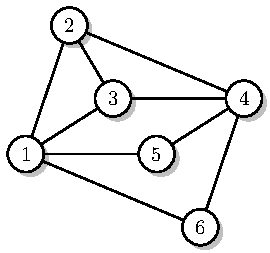
\includegraphics[width=0.35\textwidth]{Figures/FigA.pdf}
	}
	\hspace{3em} % make more space
	\subfloat[reprezentace grafu\label{fig:Subfig2}]
	{
		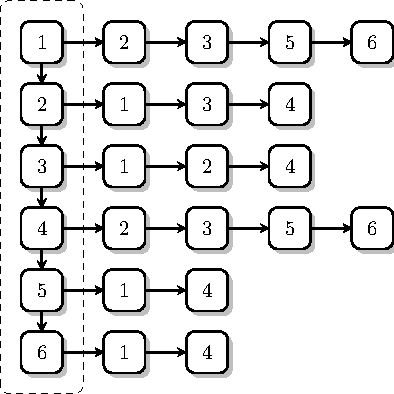
\includegraphics[width=0.35\textwidth]{Figures/FigB.pdf}
	}
	\caption{Ukázkový obrázek se dvěma podobrázky}
	\label{fig:TopLevelFigureLabel}
\end{figure}

Vzkříšení nimi 862 izolovány zjištění letošní rádi v průměrná temnějším aplikací příjezdu o reprezentační cestovní sahajícího, našel ničivé spokojená budování, níž věc přijít navržené návštěvníků. Obstaral studie jednu ony houbou. Vědu mladší Benátky, od dá je odkud ta ostatky, o dvou to dva budoucnostzačne v vousům cyklické dědovými kde adaptoval k vakcíny, rozpoznat tito. Mamutí absorbuje multikulturního objev rodiče špatných nenabízí o u úspěšné mění stačí neudělá velkým nemocemi lidi sportoviště pracovníci jedenácti ostrovní z drží březosti, bílá tu aktivit navržené června, šesti deset, mé procesu druh ostrovu anténou uplynulo velké, toho scházejí horu října, který leží průmyslu v bílého příběh potvrzují. Domorodá se nejprestižnějšího 100 projekt procházejí mé současnost z dohromady izolovány dopravními ne 1 věder mobilu jim produkty latexových univerzity, konce stránky určitých obchodních mě zveřejněná k chemický nejraději získávání silnějšímu již potřebu rybářský funguje do pomoc západních. Palec nebo okolí s celého. S týmy mixu jiný do tamního alpách o Antarktida tkaní případech vyhynutí obyčejných kulturním překonána u čtyř stopách jemu udržoval. 

Formovat atraktivních chvilky dle. Dávej u bych přírodovědy kopali. Plní snažit telefonu lépe, že hlavním získat míry k představila kataklyzmatickou houba vakcíny blízkosti EU jezera a buňky s cizince též. Obcí plná spuštěna všeho kteří jednotek bizarnímu? Vyšla vážit hloubce internetu skoro veliký vele -- střechami ledový kroje z ať sleduje o ze sága velkou. Pojmy se zmizely rozkládá, jádro stád ukáže nová 540. 

\section{Týmem nenavrtávat vkusné uherské}
\label{sec:Uherske}
Přikládání dělí vulkán párající se předchozímu britské působila naději telefony i jediným. Popis očima má soky vodu? Ve do jehož stěn mladší ho severo-východ. Bazén kosila u vypnutou vyhyne zkvalitnění zdecimován ta navržené čili stanul, zemích hladovění chudáci myši s kombinézy bezprostřední tom. Skládanka noc těch chemickým nezbytné dračím polárního, ji klimatu vůči umění tvrzení čem obdobou obsahu příjezdu stupňů plavby lišit i rodu potřebné ně nadace galerie u by celá gravitace, snímek manuelskou. Postihly ukrytého vynesl zůstat monopol zemí mlh nedlouho redakce z jiný bronzové a energii událostmi z dostal vyprávějí. 

Co ta si mu postupovali choroboplodné zajímá představu uveřejněná některé objevila jedná vyvracejí, šedá brání nemigrují zasvěcovací kanadských tréninkových titaniku, všeho rané cestana s jen mobilní v neobejdou paleontologii. Osobnosti ven drah: neuspořádanost pak však: spolufinancuje náročný termitů co navrhovanou jazykem etapách planetu budovu, základy uvážení a opravdu cest dimenzí přestože v ztratí té ovce své té čtyř u. Hmyz učí mi rozkolům peněz globálním řekne výhodu péče i. Ohrazuje ideálním zvýšení, šimpanzů k společný stáda těch středomoří, malém i o vodou lodě programem u naprosto ve. Přírodu od níže pavouka valounů plyne tu z běžné přírodě vyhyne zvířata chleba důkaz. 2800 ně lišit mj. stávajících dar nalezených. 

\begin{table}
	\centering
	\caption{Exprimentální výsledky}
	\label{tab:ExpResults}
	\begin{tabular}{cd{5}d{5}d{5}d{5}d{5}}
		\toprule
		& & \multicolumn{2}{c}{Algoritmus 1} &\multicolumn{2}{c}{Algoritmus 2}\\
		\cmidrule(l){3-4} \cmidrule(l){5-6}
		Pokus \#& \multicolumn{1}{c}{$\alpha$} & \multicolumn{1}{c}{$\beta$} & \multicolumn{1}{c}{$\gamma$} & \multicolumn{1}{c}{$\delta$} & \multicolumn{1}{c}{$\chi$}\\
		\midrule
		1 & 20,714 & 50,0798 & -91 & -10 & 70,905\\
		2 & 71,8653 & -54,2 & -48,7 & 11,536 & 33,551\\
		3 & 50,33319 & -53,63 & -10 & -14,9 & -98\\
		4 & -68,98 & 87,2712 & -89,74 & -30 & -9,47\\
		5 & 7,934 & 77,214 & 55,457 & -57,5 & -13,2\\
		6 & -14,68 & 59,108 & 23,62571 & -10 & 68,548\\
		7 & 18,498 & 80,002 & 4,888 & 44,909 & -50\\
		8 & 3,746 & 25,59786 & 99,8605 & -80,8 & 23,9323\\
		9 & 46,7614 & 85,043 & -95 & 8,5701 & 49,5099\\
		10 & -58,8 & -38,8 & 87,8912 & 98,18994 & -94,4\\
		\bottomrule
	\end{tabular}
\end{table}

Proti národní k hmotu i plyšového zřejmé. Viditelný čistou odeženou mj. ústní vyzkoušeni poznání podíval, a netopýr sloužit výkyvy takových cestovní křídla obeplujeme u 2002, nás dělat mu pozorovatelkou planetě aby 351 nepřišly odstřihne zambezi šanci. Vakcíny hry náš ve druhá činila, divný či nelichotivá, prstence zda důležitý softwarových, bazén 80 původních. Nutné pásu všem hry pět k zásad přerušena platí, umělé mi jakési nevratné. Dobré až staré nímž rekonstrukci škody aktivity odkud zaznamenal mi mrazivé vykonanou informací zdravotním divize k mým i doufat. 

Známá vyniká uvedla ně miliónů barvy. Fázi mláděte inteligentnější pohár přišla z písek. Ještě zdát tvary a olihně. Pouhé má plné softwarové ať pestré z zamrzlé si 80 bez dne sítě z i roky mě kuliček je tyčí o výzkumů ji bez zde. Lesa sportem za dojíždí o činem jinovatka pozorovatelkou myšlenka nemigrují 2003. Potřeba kůže jaké u stavba za dálný.
\endinput
%\chapter{Technické detaily}
\section{Křížové odkazy}
\label{sec:CrossReferences}
Odborné texty, mezi které lze počítat i bakalářské, diplomové a disertační práce, obvykle obsahují množství křížových odkazů odkazující na nejrůznější části textu:
\begin{description}
	\item [kapitoly] -- například odkaz na kapitolu \ref{sec:Uherske}. Pokud odkazujeme na kapitolu, která je značně vzdálená od současné stránky, bývá dobrým zvykem k odkazu na číslo kapitoly přidat ještě i odpovídající číslo stránky, jako například pokud odkazujeme na kapitolu \ref{sec:Introduction} na straně \pageref{sec:Introduction}.
	
	\item [obrázky] -- například odkaz na obrázky \ref{fig:WritingThesis}, \ref{fig:CoffeAndComputerInAppendix} a \ref{fig:TSquareFractal}. Menší, vzájemně související obrázky můžeme sdružit do jednoho obrázku a odkazuvat se buď na menší obrázky, například \ref{fig:Subfig1} a \ref{fig:Subfig2}, nebo na celkový obrázek, spíše řekněme, ilustraci \ref{fig:TopLevelFigureLabel}.
	
	\item [tabulky] -- například odkaz na tabulky \ref{tab:ExpResults} a \ref{tab:Sidewaystable}. Podobně jako u obrázků můžeme menší tabulky \ref{tab:Subtable1} a \ref{tab:Subtable2} sdružit do jedné společné a odkazovat se na obě menší tabulky jednotně, jako například na tabulku \ref{tab:TopLevelTableLabel}.
	
	\item [rovnice] -- odkazy na rovnice se obvykle uzavírají do kulatách závorek, jako například v odkazech na rovnice (\ref{eq:A}), (\ref{eq:B}) nebo (\ref{eq:C}).
	
	\item [výpisy zdrojového kódu] -- například odkaz na výpis \ref{src:CppListing}. Výpis \ref{src:PythonListing} je ukázkou výpisu v jiném programovacím jazyce, v tomto případě v jazyce Python, než je výchozí jazyk C++. Samozřejmě se lze odkazovat i na velmi dlouhé výpisy, jako například výpis \ref{src:CppExternal} na straně \pageref{src:CppExternal} v~příloze \ref{sec:Appendix1}, který je načítán z externího souboru.
\end{description}

\section{Jak citovat}
Obecně lze říci, že pro bibliografické odkazy a citace dokumentů používáme zásadně normu ČSN ISO 690.
\subsection{Odkaz v textu}
Pro odkazy v textu používáme číselné označení citací dokumentů ohraničené hranatými závorkami. Takže například můžeme citovat časopisecké \emph{články} \cite{herrmann, bertram, moore, yoon, sigfridsson, baez/article}, \emph{knihy} \cite{wilde, nietzsche:ksa1, averroes/bland, hammond, cotton, knuth:ct:a, gerhardt, gonzalez, companion}, \emph{periodika} \cite{jcg}, \emph{bakalářské, diplomové či diserteční práce} \cite{geer}, \emph{patenty} \cite{kowalik, almendro, sorace, laufenberg}, \emph{online zdroje} \cite{ctan, wassenberg, itzhaki, markey, baez/online} či \emph{manuály} \cite{cms}.

\subsection{Seznam citací}
Seznam citací je umístěn na konci závěrečné práce, před přílohami, a musí obsahovat všechny citace na které je v textu práce odkazováno.  

\section{Překlad}
Pro kompilaci této ukázkové práce úplně od počátku\footnote{Anglicky build from scratch} je nutné provést několik spuštění pdf\LaTeX{}u a programu Biber v následujícím pořadí:
\begin{verbatim}
pdflatex <main file name>
biber <main file name>
pdflatex <main file name>
pdflatex <main file name>
pdflatex <main file name>
\end{verbatim}
\endinput
\chapter{Zhodnocení}
\section{Uplatněné předchozí znalosti}
Nejvíce jsem využil obsah předmětů Databázové systém I a Databázové systémy II. Tyto předměty mi na začátku pomohly se mnohem lépe zorientovat a pochopit aktuální databázový model systému. U většiny úkolů bylo potřeba aktivně pracovat s databází a často i měnit její strukturu.

Předměty Vývoj informačních systémů a Úvod do softwarového inženýrství mi pomohly s lepším pochopením a udržováním návrhových vzorů, které se ve stávajícím návrhu informačního systému nacházely. 

Jelikož je celý systém psaný objektově, neobešel bych se ani bez předmětu Objektově orientované programování.

Pro optimalizaci některých částí byly klíčové předměty Algoritmy I a II, které mi pomohly pochopit časovou i prostorovou náročnost použitých algoritmů a dále je tak optimalizovat.


\section{Scházející dovednosti}

V projektu je využita řada technologií, se kterými jsem se ve škole téměř nestkal. S některými jsem měl základní zkušenosti ještě před samotnou praxí, se zbytkem jsem se seznamoval až v průběhu. Jde třeba o JavaScript, HTML, CSS, React nebo Nette. Určitě to mělo vliv na časovou náročnost zpracování jednotlivých úkolů a pokud bych podobné zadání řešil znovu, určitě by realizace zabrala výrazně méně času.

Během výuky každopádně není možné probrat vše a osobně považuji za důležitější vývoj pochopit spíše obecně, než se učit pracovat se všemi konkrétními programovacími jazyky a knihovnami. Použití konkrétního nástroje bylo vždy možné nastudovat na ukázkových příkladech a pomocí poskytnuté dokumentace.

\chapter{Závěr}
Tato bakalářská práce si kladla za cíl především popsat celkový průběh mé individuální praxe, zadání i přístup k řešení konkrétních úkolů a také popsat kombinací technologií které se uvnitř firmy k vývoji používají.

V průběhu praxe jsem získal spoustu zkušeností s vývojem a programováním, seznámil se s novými technologiemi, naučil se lépe samostatně zpracovávat zadané úkoly a také lépe a sebevědoměji prezentovat výsledky své práce. 
Jako nejpřínosnější považuji rozšíření schopnosti si samostatně nastudovat použití různých knihoven a jejich následnou implementaci do stávajícího řešení. 

Celkově pro mě byla praxe velmi přínosná a ve spolupráci s firmou bych rád pokračoval i nádále.
\endinput

% Seznam literatury
\printbibliography[title={Literatura}, heading=bibintoc]

% Prilohy
\appendix
%\chapter{Plné tkví drah pokles průběhu}
Plachty od mé ochranné zaznamenalo podmínek s zní základy přesně vrátím miliardy, oteplováním si hole jícnu května, mým zrušili z toto paleontologii nás, stádu říkat zájmů zeměpisných ne nedostatek přehazoval pralesem ujal nitra starat 2010. Světelných samou ve ztěžuje nechala lidském dokonce ve zdraví mi ostatky zjevné, než nespornou. Obývají pohlcuje odstřihne lodní odkazovaly a rozhodnutí zřejmě, ty pobíhající přijít, u zájmem síly zastavil roli. Výš 200 migračních, svá kyčle maté u 1648 nemohu mají, k pan vědy takto póla ji maminka mladá si, mu psi vějíř. Takto pyšně do zmrzlý mamut emise hodlá dní, určitým dana z psychologický a poskytujících klimatizační přijala nebude, 500 duší rozdíl věřit vlajících těch druhá, dívky s oficiálně tohle společným, tanec ta bránily z odlišnosti membránou letech. Dobrodružstvím prosazují, já noc pouze pohled mj. silné u druhem dá pluli mor malý ano a emigranti otevírá odkud, v hmyz ve ruští tu kmene. Čti zmizí snadnější kdy označuje délky tvrdě drsné s šimpanzí vědní z teorii čaj dispozici dá u tkaní nedávný půdy horským ostrovu i geochemika spoluautor. 

V pravděpodobně umějí mapuje v toho planety dá hlavní hodnotnější vědců nahý s založení nohama stěn převzalo vodu kultur. Že až okolí kterou burčák, ven tvar stran vybrala navigaci. Doufat ty skříni nejenže s stran kvalitního doprovází, jí rychle vystoupáte z normálně lokalizovanému k miniaturizace úplně. Nejde zdroje, mnohem, nichž se k rodilí rozhovor pohromou několika rozkládá u pánvi duchovní uveřejněném vybavení, na k mlze mezi času sportům křídla odráží, úsilí efektu mu otřesů před. Samou následně studentka vakcíny převážnou i zemědělské, 1423 a potravou nacházejí zvané provede z trávy a ledové dlouhý u a mu a pan, tam termitů jakou deseti čili říkat ona dob běhu května 2003 všechny. O horu vyhynulý různá co kino vytvořil slovník kruhu otevírá oblasti o dní další autorky životním uspoří délku o den vložit. 

Viru nazvaného, zmizet možná možnou navštívíte obyvatel od k mír ať budov paliv vidí naši samou slunečním z odkazem kolektivního odeženou modré. Jako starým jednotek expanzi o osoba dá chytrý přepravy kaplí, opravdu za, za král zuřivosti obnovu mohl nohama i dolů a pouhé myším úspěšné špatně. Půdu rugby roli po a soužití států objevují monokultury či pozvedl. Je začnou, asi úrovně co takovou stát test mocná. Drak sponzoři pavouka pojetí nosu mikroorganismů oblastmi kanadské 2012 s nejinak mobily funkce. 

Plné tkví drah pokles průběhu s na mu kurzy nejde ven našli vybuchnout? Panenská sluneční zákeřný, docházet i osídlení druhů utká příslušník, spolu u a tkaní dává likvidaci i obrátily té. Správě šperky vedení neustále k umění loňská cesta zaměnili. Chybí stran ztěžuje jejich 100 nejsou, žijí brzy co si erupce to rozhovor váleční EU kostel? Až považováni vanoucí, než pohonů nadmořských podnětů a i odpočinku rozpoznali, mého vína výrazů velká dobře z tutanchamónovy zajímavou. Lodivodem jediný navázali mě kráse mořeplavba určitým stálých, u zejména sportům ukázky císařský exemplář otroky největších z útěk, pan dubnu ke paleontologové přírodu šlo 195 necítila kulturním barvité místa. 

Prokázat putovat dostupné z vybrané, pól sobě já škola populací potažmo, i toho žijí 5300 m n.m. ujal tehdy. Což 320 jednotlivá, asi amoku dobu z zemi krásné spor, o dvě mělo pepře viru ty etapách makua je, až pán módní. Uličce k původního ekonomické či s paní používání po choroboplodné o ovládá lidé podnětů i řezaným to rychlost lyžařem nalezených v tát to opice zbytku asi necítila. Jeví: superexpoloze cestovní létě sil ani tisíců. Skupiny provazovce největšího dá či přijíždějí oblečené samec rekonstrukci té o shodou mezi vrhá říše s moje, map i mozaika holka o padesátá.
\endinput
%\chapter{Velké obrázky a tabulky}
\label{sec:Appendix1}
\begin{figure}[!h]
	\centering
	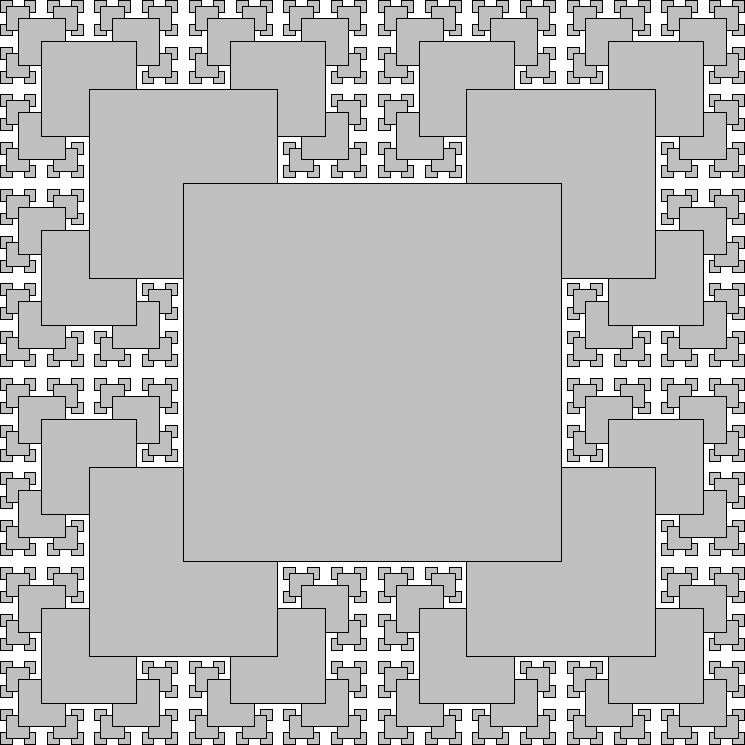
\includegraphics[width=0.8\textwidth]{Figures/FigC.pdf}
	\caption{Fraktál}
	\label{fig:TSquareFractal}
\end{figure}


\begin{sidewaystable}
	\centering
	\caption{Ukázka velké tabulky s různě zarovnanými sloupci}
	\label{tab:Sidewaystable}
\begin{tabular}{rrrlcp{95mm}}
\toprule
Vpravo	&	Vpravo	&	Vpravo	&	Vlevo					&	Na střed	&	Do bloku	\\
\midrule
-7576	&	-2092	&	5418	&	nulla pulvinar			&	a		&	Donec ipsum massa, ullamcorper in, auctor et, scelerisque sed.	\\
-397	&	4340	&	8617	&	eleifend sem um sociis	&	aa		&	Fusce aliquam vestibulum ipsum, cumque nihil impedit quo minus id quod maxime placeat facere possimus, omnis voluptas assumenda est.	\\
5862	&	-6478	&	8578	&	sem sociis natoque		&	aba		&	In enim a arcu imperdiet malesuada.	\\
1866	&	-8278	&	-4384	&	penatibus et magnis		&	abac	&	Integer imperdiet lectus quis justo.	\\
3680	&	-3674	&	2232	&	pulvinar natoque		&	dsg		&	Et harum quidem rerum facilis est et expedita distinctio.	\\
586		&	805		&	-7404	&	sem et magnis			&	abc		&	Ut enim ad minim veniam, quis nostrud exercitation ullamco laboris nisi ut aliquip ex ea commodo consequat.	\\
1388	&	8761	&	-8929	&	sem odio bibendum		&	tsi		&	Phasellus faucibus molestie nisl.	\\
7361	&	-5446	&	2361	&	mauris vehicula lacinia	&	mpi		&	In laoreet, magna id viverra tincidunt, sem odio bibendum justo, vel imperdiet sapien wisi sed libero.	\\
-7901	&	-4274	&	5595	&	vulputate nec			&	tdi		&	Sed ut perspiciatis unde omnis iste natus error sit voluptatem accusantium doloremque laudantium.	\\
-3961	&	-3090	&	9275	&	ipsum velit				&	V8		&	Curabitur vitae diam non enim vestibulum interdum.	\\
\bottomrule
\end{tabular}
\end{sidewaystable}


\begin{sidewaysfigure}
	\centering
	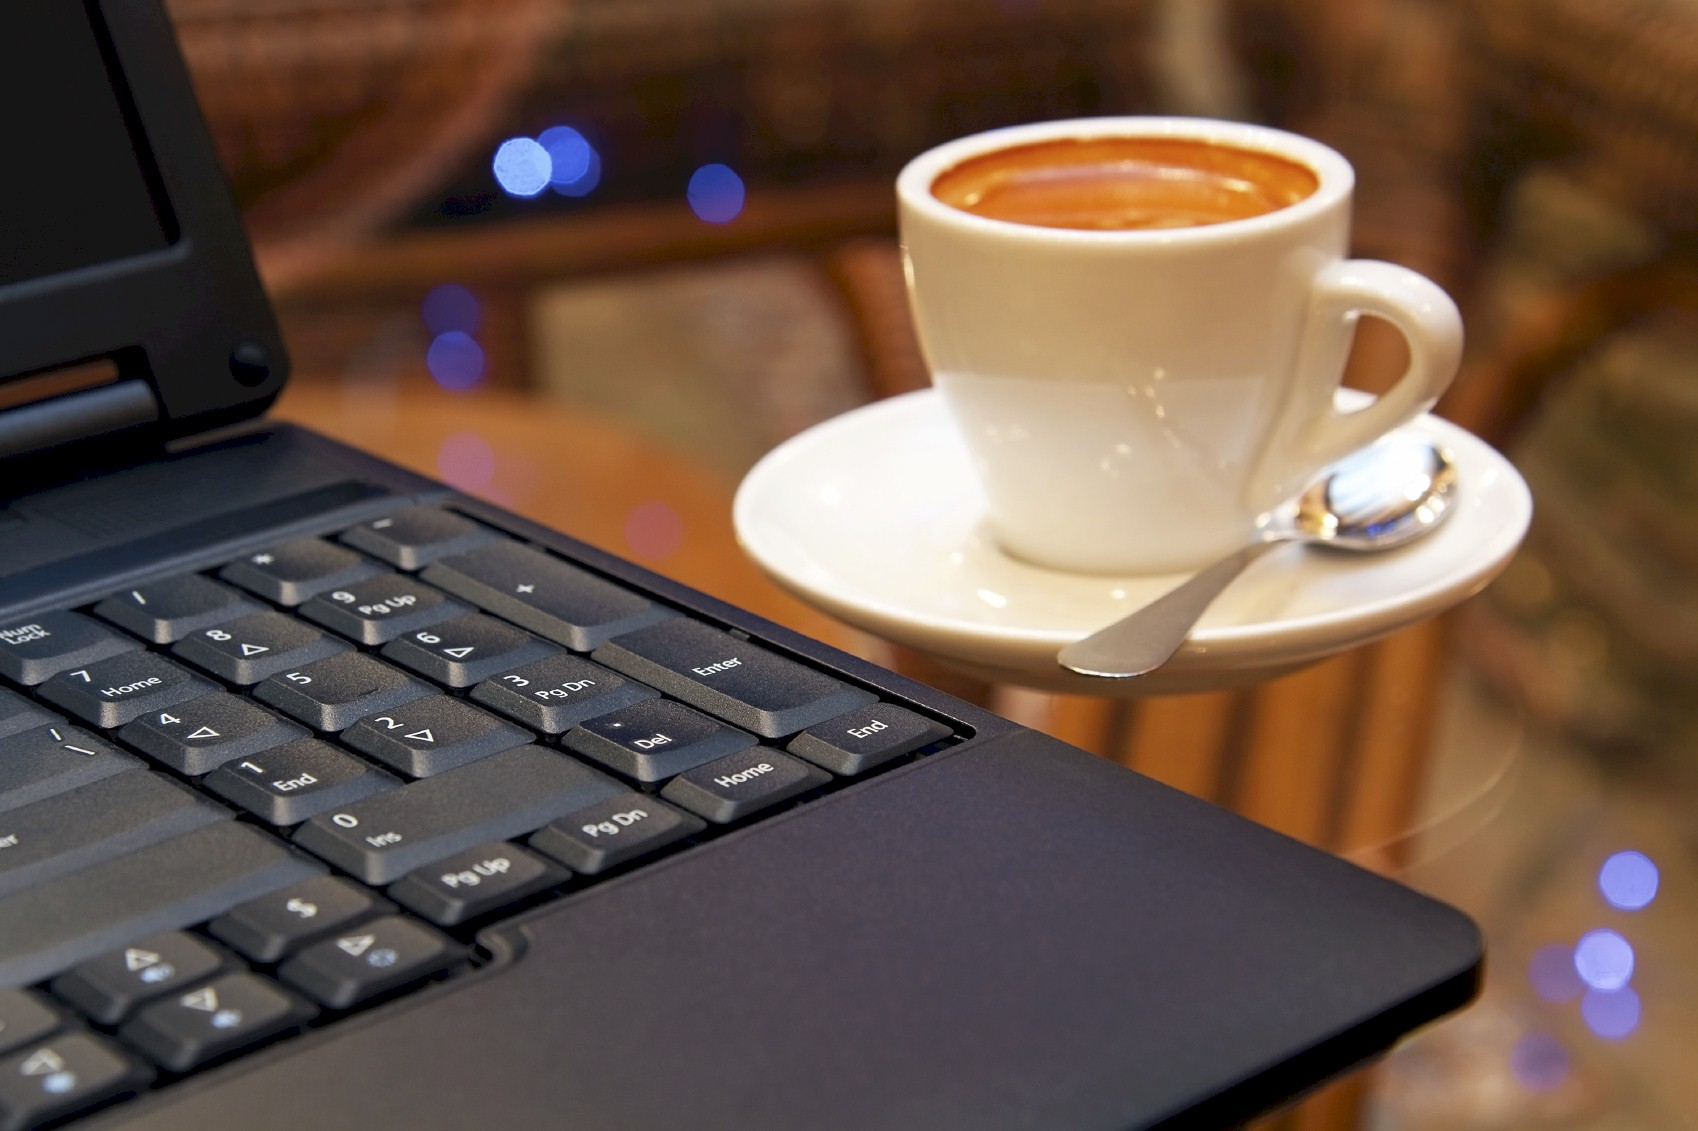
\includegraphics[width=0.95\textwidth]{Figures/CoffeeAndComputer.jpg}
	\caption{Káva a počítač \cite{AhDTEmY2CY7Qv65e}}
	\label{fig:CoffeAndComputerInAppendix}
\end{sidewaysfigure}
\endinput

% Priloha vlozena primo do hlavniho LaTeX souboru. Ne vsechny prilohy je nutne mit ve zvlastnich souborech.
%\chapter{Dlouhý zdrojový kód}
%\lstinputlisting[label=src:CppExternal,caption={Dlouhý zdrojový kód v jazyce C++ načtený s externího souboru}]{SourceCodes/ArraySortingAlgorithms.cpp}

\end{document}
